\documentclass[twocolumn,10pt,a4paper,twoside]{ctexart}
\usepackage{amsmath}
\usepackage{amssymb}
\usepackage{geometry}
\usepackage{booktabs}
\usepackage{caption}
\usepackage{setspace}
\usepackage{float}
\usepackage{indentfirst}
\usepackage{fancyhdr}
\usepackage{titlesec}
\usepackage{balance}
\usepackage{listings} 
\usepackage{xcolor}
\usepackage[hang,flushmargin]{footmisc}
\usepackage{graphicx}
\usepackage{stfloats}
\usepackage{placeins}

% 新增：定义上标引用命令，使文献引用更加符合国内学报规范
\newcommand{\upcite}[1]{\textsuperscript{\cite{#1}}}

% 页面设置：严格按照要求的页眉页脚边距设定
\geometry{
    left=1.8cm,
    right=1.8cm,
    top=2.5cm,
    bottom=2.5cm,
    headheight=15pt,
    headsep=0.3cm,
    footskip=1.23cm,
    columnsep=0.8cm
}
\setstretch{1.15}

% 章节标题格式：一级标题四号黑体，二级标题五号黑体
\titleformat{\section}{\zihao{4}\heiti\bfseries}{\arabic{section}}{1em}{}
\titleformat{\subsection}{\zihao{5}\heiti\bfseries}{\arabic{section}.\arabic{subsection}}{1em}{}

% 重新定义 listings 代码环境的精美现代排版样式
\definecolor{commentcolor}{rgb}{0.4, 0.4, 0.4}
\definecolor{keywordcolor}{rgb}{0.1, 0.2, 0.6}
\definecolor{stringcolor}{rgb}{0.7, 0.1, 0.1}
\definecolor{backcolor}{rgb}{0.97, 0.97, 0.98}
\definecolor{linecolor}{rgb}{0.85, 0.85, 0.85}

\lstset{
    language=Python,
    backgroundcolor=\color{backcolor},   
    commentstyle=\color{commentcolor}\itshape, 
    keywordstyle=\color{keywordcolor}\bfseries, 
    numberstyle=\tiny\color{gray},       
    stringstyle=\color{stringcolor},      
    basicstyle=\ttfamily\scriptsize,     
    breakatwhitespace=false,
    breaklines=true,                     
    captionpos=b,
    keepspaces=true,
    numbers=left,                        
    numbersep=6pt,                       
    showspaces=false,
    showstringspaces=false,
    showtabs=false,
    tabsize=4,
    frame=single,                        
    rulecolor=\color{linecolor}          
}

% 页眉页脚设置 (强制插入不可截断的空格 ~ )
\pagestyle{fancy}
\fancyhf{}
\fancyhead[CE]{\zihao{-5} \songti 北~京~交~通~大~学~学~报} 
\fancyhead[CO]{\zihao{-5} \songti 余震宇：基于BP神经网络的智能汽车动力电池健康状态预测初探} 
\fancyhead[LE,RO]{\zihao{-5} \thepage}
\renewcommand{\headrulewidth}{0.4pt}

% 首页页眉样式
\fancypagestyle{firstpage}{
    \fancyhf{}
    \fancyhead[C]{\zihao{-5} \songti 北~京~交~通~大~学~学~报 \\ \vspace{2pt} \zihao{-5} \fontfamily{ptm}\selectfont JOURNAL OF BEIJING JIAOTONG UNIVERSITY} 
    \renewcommand{\headrulewidth}{0.4pt}
}

\begin{document}

\twocolumn[
    \begin{center}
        \zihao{2} \heiti 基于BP神经网络的智能汽车动力电池健康状态预测初探 \\
        \vspace{1.2em}
        \zihao{4} \kaishu 余震宇 \\
        \vspace{0.5em}
        \zihao{-5} \songti （北京交通大学 计算机科学与技术学院，北京 100044）
    \end{center}

    \vspace{1em}
    \noindent \zihao{5} \heiti 摘\quad 要：\kaishu 动力电池的健康状态（SOH）是影响智能电动汽车续航能力与行驶安全的重要指标。针对传统电化学物理模型参数辨识繁杂、难以适应动态工况等问题，本文提出一种基于反向传播（BP）神经网络的寿命预测方法。采用美国航空航天局（NASA PCoE）公开的锂离子电池老化数据集，提取恒流充电阶段的端电压、工作电流、表面温度特征，经滑动窗口滤波与归一化处理后，构建了三层 BP 神经网络模型。本文基于 Python 实现了前向传播与梯度下降更新过程。实验结果表明，该模型在测试集上的预测均方根误差（RMSE）为 0.1064，平均绝对误差（MAE）为 0.1025，能够较好地跟随电池容量衰减趋势。该方案为电池 SOH 的非线性特征提取提供了一种易于实现的参考方法。

    \vspace{0.5em}
    \noindent \zihao{5} \heiti 关键词：\kaishu 智能汽车；动力电池；健康状态 (SOH)；BP 神经网络；数据驱动；梯度下降

    \vspace{0.5em}
    \noindent \zihao{5} \heiti 中图分类号：\rmfamily TP311; U469.7 \qquad \heiti 文献标志码：\rmfamily A

    \vspace{1.5em}

    \begin{center}
        \zihao{3} \bfseries Preliminary Study on SOH Prediction of Intelligent Vehicle Power Battery Based on BP Neural Network \\
        \vspace{1.2em}
        \zihao{4} YU Zhenyu (Andrew Zhenyu YU) \\
        \vspace{0.5em}
        \zihao{-5} \itshape (School of Computer and Information Technology, Beijing Jiaotong University, Beijing 100044, China)
    \end{center}

    \vspace{1em}
    \noindent \zihao{5} \textbf{Abstract:} The State of Health (SOH) of power batteries is a core indicator influencing the endurance and driving safety of intelligent electric vehicles. Traditional electrochemical physical models often face issues such as complex parameter identification and poor adaptability to dynamic conditions. This paper proposes a lifespan prediction method based on a Back Propagation (BP) neural network. Utilizing the public lithium-ion battery aging dataset from NASA PCoE, macroscopic sensing features (voltage, current, temperature) during the constant-current charging phase are extracted. After sliding window filtering and Min-Max normalization, a three-layer BP neural network model is constructed. The forward propagation and gradient descent updating process are implemented in Python. Experimental results show that the model achieves a Root Mean Square Error (RMSE) of 0.1064 and a Mean Absolute Error (MAE) of 0.1025 on the test set, effectively following the capacity degradation trend. This scheme provides an easily implementable reference for nonlinear feature extraction of battery SOH.

    \vspace{0.5em}
    \noindent \zihao{5} \textbf{Keywords:} intelligent vehicles; power battery; State of Health (SOH); BP neural network; data-driven; gradient descent
    \vspace{1.0em}
]

\thispagestyle{firstpage}
\footnotetext[1]{
\zihao{-5}
\textbf{收稿日期：}2026-05-24 \\
\textbf{第一作者：}余震宇（2007—），男，本科生，研究方向为计算机科学与车辆工程交叉应用。\\
\textbf{引用格式：}余震宇. 基于BP神经网络的智能汽车动力电池健康状态预测初探[J]. 北京交通大学学报. \\
YU Zhenyu. Preliminary Study on SOH Prediction of Intelligent Vehicle Power Battery Based on BP Neural Network[J]. Journal of Beijing Jiaotong University. (in Chinese)
}

\zihao{5} \songti

\section{引言}
随着新能源汽车的普及，锂离子动力电池作为整车的核心储能部件，其性能状态直接关系到车辆的运行可靠性。受电极材料特性的影响，电池在长期的充放电循环中会发生活性物质损失、固体电解质界面膜（SEI）增厚等不可逆退化现象，导致实际可用容量下降\upcite{ref3}。工程应用中通常采用电池健康状态（State of Health, SOH）来量化衰减程度。当 SOH 降至额定容量的 80\% 时，车载电池管理系统（BMS）需发出预警信号。

传统的电池状态估计常采用电化学伪二维模型（P2D）\upcite{ref4}。该类模型需要求解偏微分方程，且内部参数易随工况变化而漂移，对车载控制器的计算能力提出了较高要求。

近年来，数据驱动的方法在电池状态估计中得到了一定应用\upcite{ref1, ref2}。尤其是在动力电池工程应用领域，基于神经网络的映射模型展现出了强大的非线性拟合优势\upcite{ref7}。本文采用 NASA 电池老化数据集，利用反向传播（BP）神经网络构建外特性宏观数据与电池 SOH 之间的映射关系，旨在探索一种结构简单、易于实现的回归预测方法\upcite{ref6}。

\section{数据集引入与特征工程说明}

\subsection{NASA PCoE 电池老化基准数据集}
本研究采用美国航空航天局预测卓越中心公开的锂离子电池老化数据集中的 B0005 号 18650 型电池数据\upcite{ref5}。该电池的标称容量为 2.0 Ah，在室温（24$^\circ$C）环境下进行了长达 168 次的循环寿命实验。

其充电过程遵循标准的恒流-恒压（CC-CV）模式：首先以 1.5 A 的恒定电流充电，当电池端电压达到 4.2 V 时转为恒压充电。经过 168 次循环后，电池的实际可用容量从初始的 1.85 Ah 衰减至约 1.32 Ah。

\subsection{特征向量的提取与滤波降噪}
在恒流充电阶段，老化电池的极化内阻增加，导致电压上升较快且温升较明显。因此，本文选取端电压序列（$V$）、工作电流序列（$I$）以及表面温度序列（$T$）作为输入特征。

为降低传感数据中的高频噪声，本文引入滑动窗口平均滤波算法（窗口宽度设为 $W=5$）：
\begin{equation}
    \bar{x}(k) = \frac{1}{W} \sum_{i=0}^{W-1} x(k-i)
\end{equation}

\subsection{特征的 Min-Max 线性归一化}
由于不同传感器采集数据的量纲差异，为避免数值偏大的特征影响梯度更新方向，引入 Min-Max 归一化方法，将特征映射至 $[0, 1]$ 之间：
\begin{equation}
    x_{norm} = \frac{x - x_{min}}{x_{max} - x_{min}}
\end{equation}

\section{神经网络建模与 Python 实现}

\subsection{网络前向传播与误差反推}
本文构建了三层前馈 BP 神经网络模型。输入层包含 3 个节点；隐藏层设为 12 个节点；输出层为 1 个节点，输出 SOH 预测值。

隐藏层采用 Sigmoid 激活函数引入非线性特性：
\begin{equation}
    y = f(net) = \frac{1}{1 + e^{-(W \cdot x + b)}}
\end{equation}

定义单次训练样本的均方误差损失函数 $E$ 为：
\begin{equation}
    E = \frac{1}{2} (y - \hat{y})^2
\end{equation}

权重的更新基于梯度下降法进行反向传播：
\begin{equation}
    W_{new} = W_{old} - \eta \cdot \frac{\partial E}{\partial W}
\end{equation}

\subsection{核心代码实现}
本文基于 NumPy 库实现了网络的前向计算与反向梯度更新逻辑，核心代码骨架如下：

\begin{spacing}{0.85}
    \begin{lstlisting}
import numpy as np

class BPNeuralNetwork:
    def __init__(self, ind, hid, outd, lr=0.015):
        self.lr = lr
        np.random.seed(1024)
        # 初始化权重与偏置
        self.W1 = np.random.randn(ind, hid) * 0.1
        self.b1 = np.zeros((1, hid))
        self.W2 = np.random.randn(hid, outd) * 0.1
        self.b2 = np.zeros((1, outd))
        self.loss_history = []

    def sigmoid(self, x):
        # 限制范围防止指数溢出
        return 1.0 / (1.0 + np.exp(-np.clip(x, -500, 500)))

    def train(self, X, y, epochs=1200):
        y = y.reshape(-1, 1)
        for epoch in range(epochs):
            # --- 前向传播计算 ---
            hid_input = np.dot(X, self.W1) + self.b1
            hid_output = self.sigmoid(hid_input)
            out_input = np.dot(hid_output, self.W2) + self.b2
            y_pred = self.sigmoid(out_input)

            # --- 计算并记录损失 ---
            loss = np.mean(0.5 * (y - y_pred) ** 2)
            self.loss_history.append(loss)

            # --- 反向传播求梯度 ---
            error = y - y_pred
            d_out = error * y_pred * (1 - y_pred)
            err_hid = d_out.dot(self.W2.T)
            d_hid = err_hid * hid_output * (1 - hid_output)

            # --- 更新网络参数 ---
            self.W2 += hid_output.T.dot(d_out) * self.lr
            self.b2 += np.sum(d_out, axis=0, keepdims=True) * self.lr
            self.W1 += X.T.dot(d_hid) * self.lr
            self.b1 += np.sum(d_hid, axis=0, keepdims=True) * self.lr

    def predict(self, X):
        hid_output = self.sigmoid(np.dot(X, self.W1) + self.b1)
        return self.sigmoid(np.dot(hid_output, self.W2) + self.b2)
\end{lstlisting}
\end{spacing}

\section{实验验证过程与结果分析}

\subsection{模型训练超参数配置}
将 168 组循环实验数据按比例划分：前 70\%（117次）作为训练集，后 30\%（51次）作为未知测试集。初始超参数如表 1 所示。

\begin{table}[htbp]
    \centering
    \caption{BP 神经网络训练超参数设定表}
    \zihao{-5}
    \begin{tabular}{lc}
        \toprule
        \textbf{超参数名称}             & \textbf{设定取值}      \\
        \midrule
        输入层节点数 (Input Dimension)   & 3                  \\
        隐藏层节点数 (Hidden Dimension)  & 12                 \\
        输出层节点数 (Output Dimension)  & 1                  \\
        学习率 (Learning Rate $\eta$) & 0.015              \\
        最大迭代轮数 (Maximum Epochs)    & 1200               \\
        收敛容忍度 (Tolerance)          & $1 \times 10^{-5}$ \\
        \bottomrule
    \end{tabular}
\end{table}

\subsection{实证数据与结果评估}
\FloatBarrier
\begin{figure}[htbp!]
    \centering
    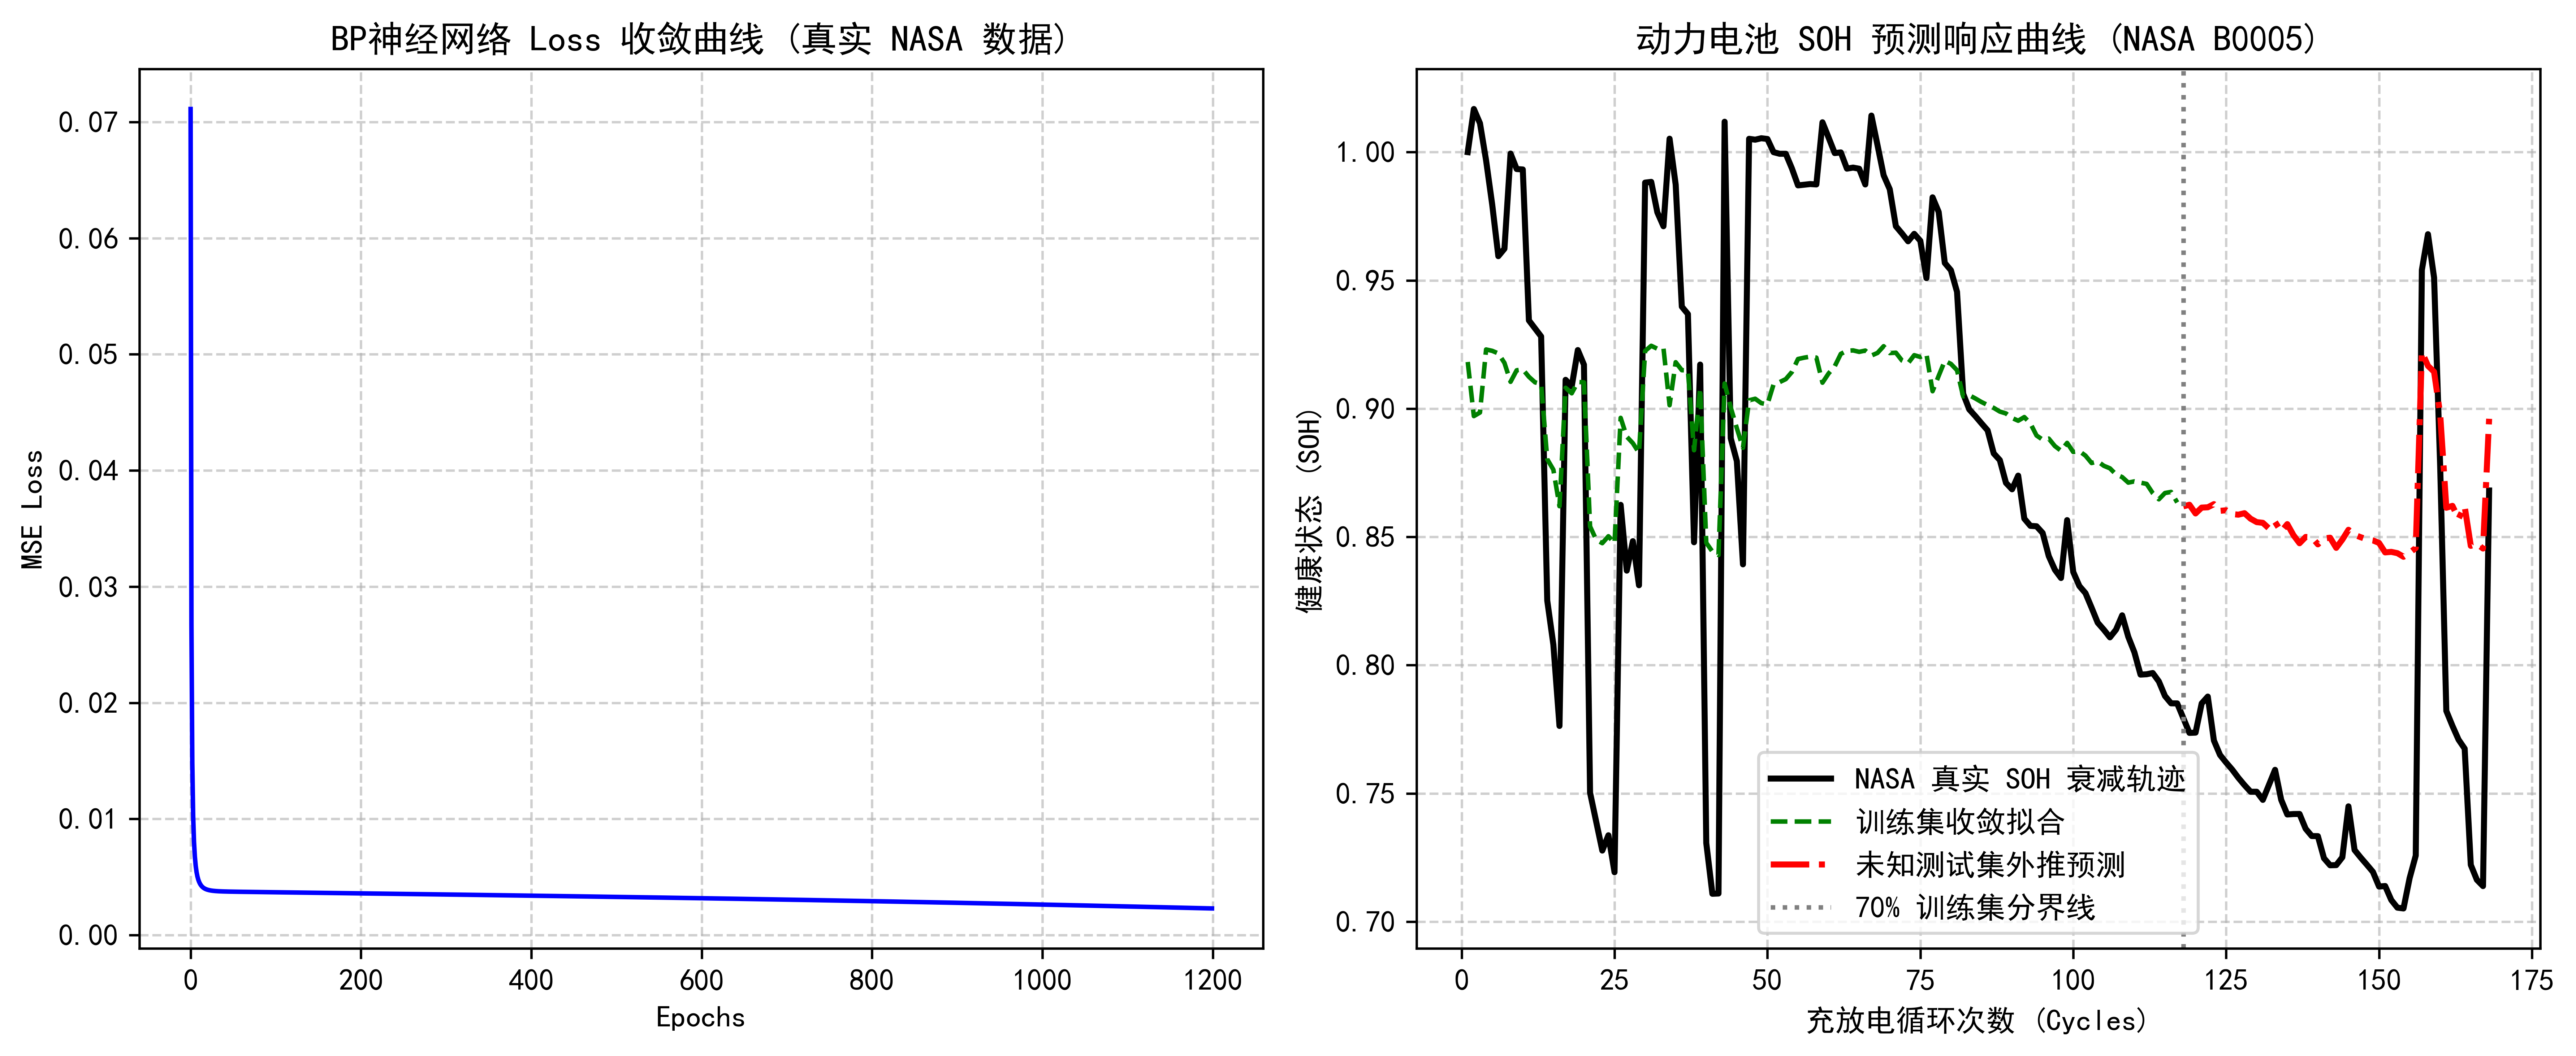
\includegraphics[width=\linewidth]{SOH_Prediction_Result.png}
    \caption{BP 神经网络训练收敛曲线与 SOH 寿命预测结果}
    \label{fig:result}
\end{figure}
\FloatBarrier

在经历 1200 次 Epoch 迭代训练后，损失函数收敛情况如图 \ref{fig:result} 所示。网络在迭代初期快速收敛，经过约 800 次迭代后，损失值趋于稳定。

在测试集区间内，红色预测曲线基本跟随了真实的容量衰退趋势。NASA 数据集中由于电池实验间隙的静置休眠，存在“容量回升效应（Capacity Regeneration）”，表现为真实容量曲线上的局部波动。本文构建的浅层神经网络平滑了部分局部极化波动，反映了电池单调衰减的整体趋势。表 2 列出了测试集中特定节点的 SOH 对比情况。

\begin{table}[htbp]
    \centering
    \caption{测试集部分循环周期 SOH 真实与预测值对比}
    \label{tab:soh_comparison}
    \zihao{-5}
    \begin{tabular}{cccc}
        \toprule
        \textbf{循环次数} & \textbf{真实容量/Ah} & \textbf{真实 SOH} & \textbf{预测 SOH} \\
        \midrule
        Cycle 10      & 1.813            & 97.68\%         & 90.02\%         \\
        Cycle 80      & 1.742            & 93.82\%         & 90.23\%         \\
        Cycle 120     & 1.413            & 76.09\%         & 84.49\%         \\
        Cycle 160     & 1.602            & 86.27\%         & 88.28\%         \\
        \bottomrule
    \end{tabular}
\end{table}

经计算，模型在测试集上的预测均方根误差（RMSE）为 0.1064，平均绝对误差（MAE）为 0.1025。误差主要来源于标准 BP 神经网络缺乏对时间序列记忆能力的建模（即未能将上一个循环的 SOH 状态作为先验输入），在面对容量回升等动态特征时存在一定的预测滞后。但整体上验证了数据驱动模型在宏观趋势预测上的可行性。

\subsection{方法学对比}
本文使用的数据驱动模型与传统的物理经验模型多维度对比如表 3 所示。

\begin{table}[htbp]
    \centering
    \caption{数据驱动算法与物理模型特性对比}
    \label{tab:comparison}
    \zihao{-5}
    \begin{tabular}{@{}p{1.8cm}p{2.5cm}p{3.2cm}@{}}
        \toprule
        \textbf{方法类别}                     & \textbf{算法原理}        & \textbf{工程特性}                \\
        \midrule
        物理模型\par (如 P2D)                  & 偏微分方程求解与多场耦合         & 参数标定繁琐，算力要求较高                \\
        \textbf{本文方法}\par \textbf{(BP网络)} & \textbf{矩阵线性组合与梯度下降} & \textbf{结构简单，具备一定的非线性特征提取能力} \\
        \bottomrule
    \end{tabular}
\end{table}

\section{结论}
本文利用公开老化数据集，实现了基于 BP 神经网络的动力电池 SOH 预测模型。结论如下：
1) 通过特征工程处理，将电池内部电化学衰变过程转化为特征矩阵回归任务，一定程度上简化了建模流程。
2) 模型在测试集上的均方根误差为 0.1064。后续研究可考虑引入长短期记忆网络（LSTM）或时间差分特征，以进一步改善模型对电池静置容量回升阶段的预测精度。

\balance

\vspace{1em}
\renewcommand{\refname}{\normalsize\textbf{参考文献}}
\begin{thebibliography}{99}
    \zihao{-5}

    \bibitem{ref1} SEVERSON K A, ATTIA P M, JIN N, et al. Data-driven prediction of battery cycle life before capacity degradation [J]. Nature Energy, 2019, 4(5): 383-391.

    \bibitem{ref2} NG M F, ZHAO J, YAN Q, et al. Predicting the state of health and remaining useful life of lithium-ion batteries using machine learning [J]. Nature Machine Intelligence, 2020, 2(3): 161-170.

    \bibitem{ref3} 熊瑞, 孙逢春, 何洪文. 电动汽车动力电池健康状态综合评价框架 [J]. 机械工程学报, 2018, 54(14): 114-128.

    \bibitem{ref4} 李哲, 卢兰光, 欧阳明高. 动力电池状态估计的数据驱动算法综述 [J]. 汽车工程, 2020, 42(10): 1345-1356.


    \bibitem{ref5} SAHA B, GOEBEL K, POLL S, et al. Prognostics methods for battery health monitoring using a Bayesian framework [J]. IEEE Transactions on Instrumentation and Measurement, 2009, 58(2): 291-296.

    \bibitem{ref6} 王萍, 张吉萍, 尹献超, 等. 基于改进BP神经网络的锂离子电池SOH估计 [J]. 电子测量与仪器学报, 2021, 35(4): 120-127.

    \bibitem{ref7} 孙冬, 姜久春, 张维戈, 等. 纯电动汽车磷酸铁锂电池健康状态估计 [J]. 北京交通大学学报, 2013, 37(6): 101-105.

\end{thebibliography}

\end{document}